\chapter{Formulation pratique d'éléments finis \pln}\label{Ch-Elts}
\begin{abstract}
L'intégralité de la méthode des éléments finis a été présentée au chapitre~\ref{Ch-MEF}.

Dans ce chapitre et dans les suivants, nous allons détailler certains aspects.
Nous proposons dans ce chapitre d'exposer un peu plus complètement les notions
d'interpolation sur un élément, ainsi que le lien entre approximation locale
(sur un élément) et approximation globale (construction de la base de $V_h$).
\end{abstract}


Nous avons dit vouloir interpoler le problème sur chaque élément.
Pour ce faire, il faut prendre une \textcolorblue{base} sur chaque élément.
Plusieurs choix sont possibles, mais en général, les fonctions de base utilisées pour les
éléments finis sont dites \textcolorblue{interpolantes}, c'est-à-dire que les
\textcolorblue{valeurs nodales} sont les valeurs des grandeurs inconnues aux nœuds,
et que c'est à partir de ces valeurs que l'on effectue l'interpolation.

\medskip
La méthode la plus simple consiste à utiliser les polynômes de Lagrange.\index[aut]{Lagrange (Joseph Louis, comte de -), 1736-1813, Italien}
Dans cette méthode les fonctions de base valent 1 à un nœud du maillage et 0 à tous les autres.
La fonction de base $i$ est alors la fonction valant 1 au nœud $i$ et 0 sur les autres nœuds
et qui est polynomiale sur chaque élément.
Il y a autant de fonctions de base par élément que de nombre de nœuds.

On appelle \textcolorblue{élément} la donnée d'une \textcolorblue{géométrie}
(souvent polygonale en 2D, polyédrique en 3D) et de \textcolorblue{fonctions de base associées
à cette géométrie}.

\medskip
D'autres solutions peuvent exister pour les fonctions de base.
Par exemple, les éléments finis d'Hermite\index[aut]{Hermite (Charles), 1822-1901, Français}
ont la particularité d'avoir deux fonctions de base associées à chaque nœud.
La valeur de la solution est alors ajustée avec la première fonction alors que la deuxième
permet d'ajuster la valeur de la dérivée.
Ce type de fonctions de base peut avoir un intérêt pour la résolution de certaines EDP
(telle que l'équation des plaques en MMC), même si elle nécessite d'avoir deux fois plus
de fonctions pour un maillage donné.








\medskip
\section{Éléments de Lagrange}\index{EF de Lagrange}\index[aut]{Lagrange (Joseph Louis, comte de -), 1736-1813, Italien}

Les éléments de Lagrange sont les éléments finis les plus simples.

\medskip
\subsection{Unisolvance}\index{Unisolvance}\label{Sec-unisolvance}

\begin{definition}[Unisolvance]
Soit $\Sigma=\{a_1,\ldots, a_N\}$ un ensemble de $N$ points distincts de $\RR^n$.
Soit $P$ un espace vectoriel de dimension finie de fonctions de $\RR^n$ à valeurs dans $\RR$.
On dit que $\Sigma$ est \textcolorblue{$P$-unisolvant} ssi pour tous réels $\alpha_1$,\ldots, $\alpha_N$,
il existe un unique élément $p$ de $P$ tel que $\forall i=1,\ldots, N$, $p(a_i) = \alpha_i$.
(ce qui revient à dire que la fonction de $P$ dans $\RR^N$ qui à $p$ fait correspondre
$(p(a_i),\ldots, p(a_N))=(\alpha_1,\ldots, \alpha_N)$ est bijective).
\end{definition}

\medskip
\subsection{Éléments finis de Lagrange}\index{EF de Lagrange}

\begin{definition}[Éléments finis de Lagrange]
Un \textcolorblue{élément fini de Lagrange} est un triplet $(K, \Sigma, P)$ tel que:
\begin{itemize}
\item $K$ est un élément géométrique de $\RR^n$, compact, connexe, et d'intérieur
	non vide;
\item $\Sigma=\{a_1,\ldots, a_N\}$ un ensemble de $N$ points distincts de $\RR^n$;
\item $P$ est un espace vectoriel de dimension finie de fonctions réelles définies sur $K$, et tel
	que $\Sigma$ soit $P$-unisolvant (donc $\dim P = N$).
\end{itemize}
\end{definition}

\medskip
Les \textcolorblue{fonctions de bases locales} de l'élément fini de Lagrange $(K, \Sigma, P)$
sont les $N$ fonctions de $P$ telles que $p_i(a_j)=\delta_{ij}$ pour $1\le i,j\le N$.

\medskip
\paragraph{Remarque} $(p_1,\ldots, p_N)$ est une base de $P$.

\medskip
\begin{definition}[Opérateur de $P$-interpolation]
Un \textcolorblue{opérateur de $P$-interpolation sur $\Sigma$} est un opérateur $\pi_K$
qui à toute fonction $v$ définie sur $K$ associe la fonction $\pi_Kv$ de $P$ définie par:
$\pi_Kv=\dsum_{i=1}^N v(a_i)p_i$.
\end{definition}

\begin{theoreme}
$\pi_kv$ est l'unique élément de~$P$ qui prend les mêmes valeurs que~$v$ sur les
points de~$\Sigma$.
\end{theoreme}

\medskip
On notera \textcolorblue{$P_k$ l'espace vectoriel des polynômes de degré total inférieur ou égal à $k$.}
\begin{itemize}
\item sur $\RR$, $P_k=Vect\{1, X,\ldots, X^k\}$ et $\dim P_k=k+1$;
\item sur $\RR^2$, $P_k=Vect\{X^iY^j, 0\le i+j\le k\}$ et $\dim P_k=\frac{(k+1)(k+2)}2$;
\item sur $\RR^3$, $P_k=Vect\{X^iY^jZ^l, 0\le i+j+l\le k\}$ et $\dim P_k=\frac{(k+1)(k+2)(k+3)}6$.
\end{itemize}
\medskip
On notera \textcolorblue{$Q_k$ l'espace vectoriel des polynômes de degré inférieur ou égal à $k$ par rapport
à chaque variable.}
\begin{itemize}
\item sur $\RR$, $Q_k=P_k$;
\item sur $\RR^2$, $Q_k=Vect\{X^iY^j, 0\le i,j\le k\}$ et $\dim Q_k=(k+1)^2$;
\item sur $\RR^3$, $Q_k=Vect\{X^iY^jZ^l, 0\le i,j,l\le k\}$ et $\dim Q_k=(k+1)^3$.
\end{itemize}



\medskip
\subsection*{Éléments finis unidimensionnels}

On discrétise le segment $[a,b]$ avec des polynômes de degrés $1$ à $m$.
On obtient les éléments du tableau~\ref{tab:Elem:uni}.
\begin{table}[ht]\centering\small
\begin{tabular}{c|cccc}
Élément & $P_1$ & $P_2$ & ... & $P_m$\\
\hline
$K$	      & $[a,b]$ &  $[a,b]$ & ... & $[a,b]$\\
$\Sigma$   & $\{a,b\}$ & $\{a,\frac{a+b}2, b\}$& ... &$\{a+i\frac{b-a}m, i=0,\ldots, m\}$\\
$P$            & $P_1$ & $P_2$ & ... & $P_m$\\
\hline
\end{tabular}
\caption{}\label{tab:Elem:uni}
\end{table}

\medskip
\subsection*{Éléments finis bidimensionnels triangulaires}
On discrétise le triangle de sommets $\{a_1, a_2, a_3\}$ avec, le long de chaque
arête une interpolation polynomiale de degré $1$ à $m$.
On obtient les éléments du tableau~\ref{tab:Elem:bi}.
\begin{table}[ht]\centering\small
\begin{tabular}{c|cc}
Élément & $P_1$ & $P_2$ \\
\hline
$K$	      & triangle de sommets $\{a_1, a_2, a_3\}$ & triangle de sommets $\{a_1, a_2, a_3\}$\\
$\Sigma$   & $\{a_1, a_2, a_3\}$ & $\{a_{ij}=\frac{a_i+a_j}2, 1\le i,j\le 3\}$ \\
$P$            & $P_1$ & $P_2$ \\
\hline
\end{tabular}
\caption{}\label{tab:Elem:bi}
\end{table}

\paragraph{Remarque}Les fonctions de base pour l'élément $P_1$ sont définies par $p_i(a_j) = \delta_{ij}$. Ce sont les coordonnées barycentriques: $p_i = \lambda_i$.

\medskip
\subsection*{Éléments finis bidimensionnels rectangulaires}
On discrétise le rectangle de sommets $\{a_1, a_2, a_3, a_4\}$ de côtés
parallèles aux axes. La formulation est décrite dans le tableau~\ref{tab:Elem:bibi}.
\begin{table}[ht]\centering\small
\begin{tabular}{c|c}
Élément & $Q_1$\\
\hline
$K$ & rectangle de sommets $\{a_1, a_2, a_3, a_4\}$ de côtés parallèles aux axes.\\
$\Sigma$ & $\{a_1, a_2, a_3, a_4\}$\\
$P$ & $Q_1$\\
\hline
\end{tabular}
\caption{}\label{tab:Elem:bibi}
\end{table}

\begin{figure}[ht]
\centering
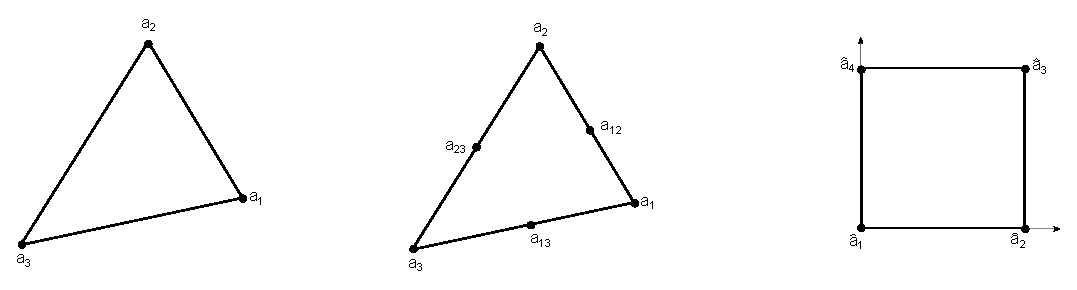
\includegraphics[height=30mm]{Lagrange2D.eps}
\caption{\label{Lagrange2D} Éléments finis de Lagrange 2D: triangulaire $P_1$, triangulaire $P_2$ et rectangulaire $Q_1$}
\end{figure}

\medskip
\subsection*{Éléments finis tridimensionnels}
Les éléments tétraédriques sont définis dans le tableau~\ref{tab:Elem:tri}.
\begin{table}[ht]\centering\small
\begin{tabular}{c|cc}
Élément & $P_1$ & $P_2$ \\
\hline
$K$	      & tétraèdre de sommets $\{a_1, a_2, a_3, a_4\}$ & tétraèdre de sommets $\{a_1, a_2, a_3, a_4\}$\\
$\Sigma$   & $\{a_1, a_2, a_3, a_4\}$ & $\{a_i\}_{1\le i\le4}\cup\{a_{ij}\}_{1\le i<j\le 4}$ \\
$P$            & $P_1$ & $P_2$ \\
\hline
\end{tabular}
\caption{}\label{tab:Elem:tri}
\end{table}

Élément parallélépipédique [tableau~\ref{tab:Elem:para}].
\begin{table}[ht]\centering\small
\begin{tabular}{c|c}
Élément & $Q_1$\\
\hline
$K$ & parallélépipède de sommets $\{a_1,\ldots, a_8\}$ de côtés parallèles aux axes.\\
$\Sigma$ & $\{a_i\}_{1\le i\le8}$\\
$P$ & $Q_1$\\
\hline
\end{tabular}
\caption{}\label{tab:Elem:para}
\end{table}

Élément prismatique [tableau~\ref{tab:Elem:pri}].
\begin{table}[ht]\centering\small
\begin{tabular}{c|c}
Élément & $Q_1$\\
\hline
$K$ & prisme droit de sommets $\{a_1,\ldots, a_6\}$\\
$\Sigma$ & $\{a_i\}_{1\le i\le6}$\\
$P$ & $\{p(X,Y,Z) = (a + bX + cY ) + Z(d + eX + fY ), a,b,c,d,e,f\in\RR\}$\\
\hline
\end{tabular}
\caption{}\label{tab:Elem:pri}
\end{table}
\begin{figure}[ht]
\centering
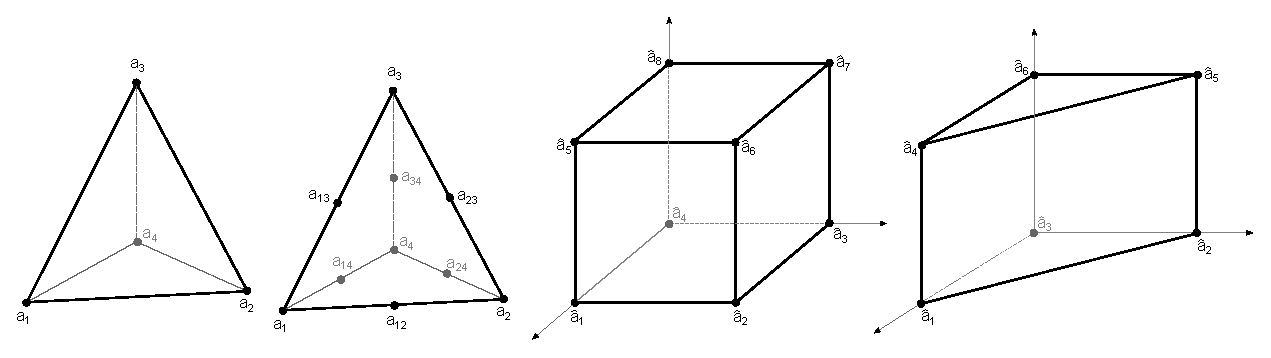
\includegraphics[width=\textwidth]{Lagrange3D.eps}
\caption{Éléments finis de Lagrange 3D: tétraédriques $P_1$ et $P_2$, parallélépipédique $Q_1$ et prismatique}\label{Lagrange3D}
\end{figure}



\medskip
\subsection{Famille affine d'éléments finis -- élément de référence}\index{Elément de référence}\index{Famille affine d'EF}

En fait, la notion de transformation affine entre un élément $K$ d'un maillage
$\mathcal{T}_h$ et un élément de référence a déjà été utilisée en
calcul de majoration d'erreur, mais la transformation elle-même n'a pas été
détaillée.

\medskip\colorgris
Deux éléments finis $(\hat{K}, \hat{\Sigma}, \hat{P})$ et $(K, \Sigma, P)$ sont
affine-équivalents ssi il existe une fonction affine $F$ inversible telle que
$K=F(\hat{K})$, $a_i=F(\hat{a_i})$, i=1,\ldots, N, et $P=\{\hat{p}\circ F^{-1}, \hat{p}\in\hat{P}\}$.
\colorblack\normalsize

\medskip
\begin{definition}[famille affine d'éléments finis]
On appelle \textcolorblue{famille affine d'éléments finis} une famille d'éléments finis
tous affine-équivalents à un même EF appelé \textcolorblue{élément
de référence}.
\end{definition}

\medskip
\textcolorgreen{D'un point de vue pratique, le fait de travailler avec une famille affine d'EF permet
de ramener tous les calculs d'intégrales à des calculs sur l'élément de référence.}
Voir figure \ref{trsfaffine} pour une illustration d'une transformation affine.
\begin{figure}[ht]
\centering
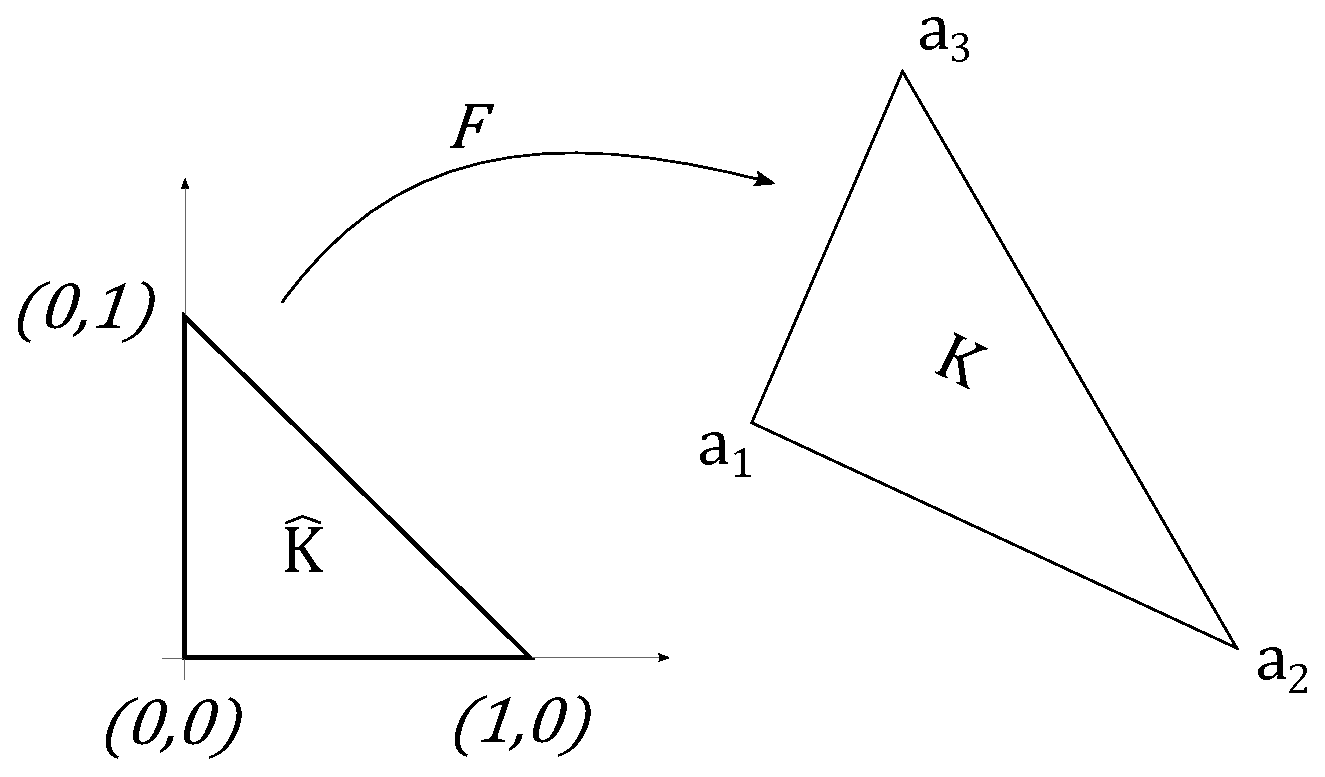
\includegraphics[height=45mm]{trsfaffine.eps}
\caption{\label{trsfaffine} Transformation affine sur un triangle}
\end{figure}

\medskip
Les EF de références sont ceux obtenus, dans les cas présentés ci-dessus avec:
\begin{itemize}
\item le segment $[0,1]$ en 1D;
\item le triangle unité de sommets $(0,0)$, $(0,1)$, $(1,0)$,
\item et le carré unité $[0,1]\times[0,1]$ en 2D;
\item le tétraèdre unité de sommets $(0,0,0)$, $(1,0,0)$, $(0,1,0)$, $(0,0,1)$,
\item le cube unité $[0,1]\times[0,1]\times[0,1]$,
\item le prisme unité de sommets $(0,0,0)$, $(0,1,0)$, $(1,0,0)$, $(0,0,1)$, $(0,1,1)$, $(1,0,1)$.
\end{itemize}



\medskip
\subsection{Construction de la base globale}

Revenons à notre problème décrit par une EDP sous forme faible dans un domaine
$\Omega$ sur lequel on réalise un maillage $\mathcal{T}_h$ à partir d'une famille affine
de $N_e$ éléments finis $(K_i, \Sigma_i, P_i)_{i=1,\ldots,N_e}$.

\medskip
Par unisolvance, la solution approchée $u_h$ sera entièrement définie sur chaque EF
par ses valeurs sur les points de $\Sigma_i$, nommés \textcolorblue{nœuds} du maillage.
Notons $(a_1,\ldots, a_{N_h})$ les nœuds du maillage ($N_h<N_e . Card\Sigma_i$).
Le problème approché revient à déterminer les valeurs de $u_h$ aux points $a_i$:
ce sont les \textcolorblue{degrés de liberté} du problème approché.

\medskip
On va construire une base de $V_h$ en associant à chaque ddl $a_i$ un vecteur de la base.
On définit ainsi les fonctions de base globales $\varphi_i$ $(i = 1,\ldots, N_h)$ par:
\begin{equation}\varphi_i|_{K_j} \in P_j, j = 1,\ldots, N_e \quad \text{ et }\quad \varphi_i(a_j) = \delta_{ij}, 1\le i,j\le N_h\end{equation}
et l'espace d'approximation interne est: $V_h=Vect\{\varphi_1,\ldots, \varphi_{N_h}\}$.

On remarquera qu'une telle fonction $\varphi_i$ est nulle partout sauf sur les éléments
dont $a_i$ est un nœud.
\begin{figure}[ht]
\centering
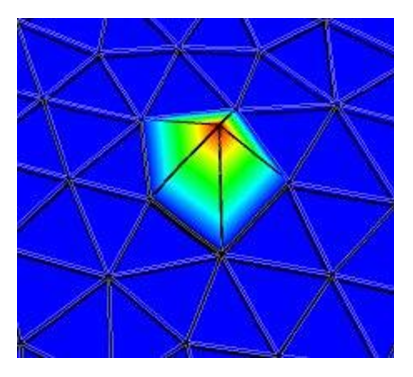
\includegraphics[height=40mm]{phi1}~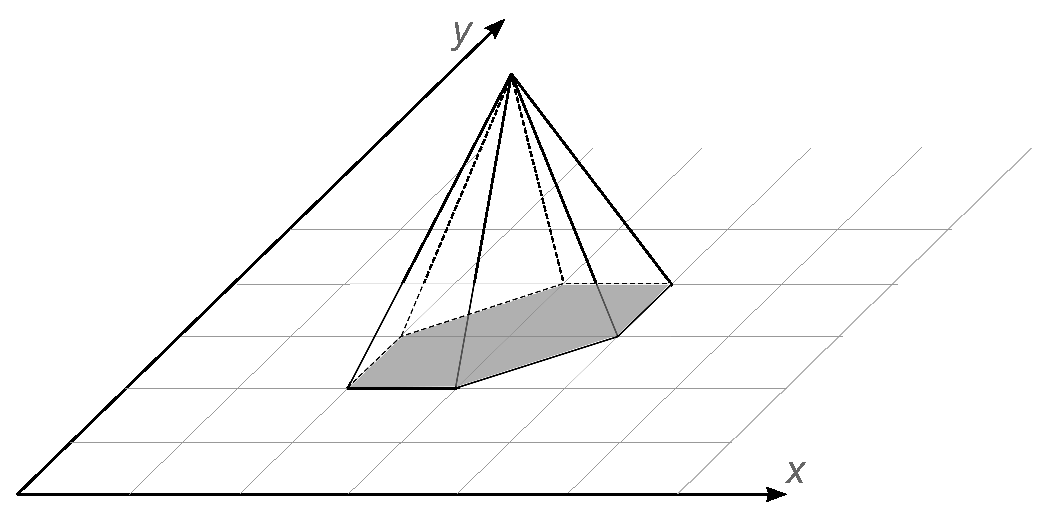
\includegraphics[height=40mm]{phi2.eps}
\caption{\label{BaseVh} Base de $V_h$: exemple de fonction de base globale $\varphi_i$ sur un maillage avec des éléments triangulaires $P_1$.}
\end{figure}

\medskip
De plus, sur un élément $K$ dont $a_i$ est un nœud, $\varphi_i$ vaut $1$ en $a_i$ et
$0$ aux autres nœuds de K. Donc $\varphi_i|_K$ est une fonction de base locale de $K$.
On voit donc que la fonction de base globale $\varphi_i$ est construite comme réunion des
fonctions de base locales sur les éléments du maillage dont $a_i$ est un nœud.

\medskip
Remarque: ce qui précède est vrai dans le cas d'un maillage conforme, i.e si
l'intersection entre deux éléments est soit vide, soit réduite à un
sommet ou une arête en dimension 2, ou à un sommet, une arête ou une face
en dimension 3.
\begin{figure}[ht]
\centering
\includegraphics[height=25mm]{MaillageNC.eps}
\caption{\label{maillageNC} Maillage non conforme: situations interdites}
\end{figure}

\medskip
\section{Éléments d'Hermite}\index{EF d'Hermite}\index[aut]{Hermite (Charles), 1822-1901, Français}

\medskip
\subsection{Classe d'un EF}\index{Classe d'un EF d'Hermite}\index[aut]{Hermite (Charles), 1822-1901, Français}

Une question naturelle est de savoir quelle est la régularité de la solution approchée
$u_h$. En particulier, $u_h$ est-elle continue? dérivable?

$u_h$ est obtenue par combinaison linéaire des fonctions de base globales
$\varphi$, la question revient donc à déterminer la régularité de celles-ci.
Par construction, on voit que la régularité de $\varphi_i$ sera donnée par sa
régularité au niveau des interfaces entre les éléments adjacents formant
son support.

Dans les EF de Lagrange, $\varphi_i$ est construite pour être continue
d'un élément à l'autre, mais pas sa dérivée... c'est cette contrainte que
nous allons introduire maintenant.

\medskip
\subsection{EF d'Hermite}\index{EF d'Hermite}\index[aut]{Hermite (Charles), 1822-1901, Français}

\begin{definition}[EF d'Hermite]
Un \textcolorblue{élément fini d'Hermite ou élément fini général} est un
triplet $(K, \Sigma, P)$ tel que:
\begin{itemize}
\item $K$ est un élément géométrique de $\RR^n$, compact, connexe, et d'intérieur
	non vide;
\item $\Sigma=\{\sigma_1,\ldots, \sigma_N\}$ un ensemble de $N$ \textcolorred{formes linéaires}
	sur l'espace des fonctions définies sur $K$, ou sur un sous-espace plus régulier contenant $P$;
\item $P$ est un espace vectoriel de dimension finie de fonctions réelles définies sur $K$, et tel
	que $\Sigma$ soit $P$-unisolvant.
\end{itemize}
\end{definition}

\medskip
\begin{definition}[Opérateur de P-interpolation]
Un \textcolorblue{opérateur de P-interpolation sur $\Sigma$} est un opérateur $\pi_K$
qui à toute fonction $v$ définie sur $K$ associe la fonction $\pi_Kv$ de $P$ définie par:
$\colorred\pi_Kv=\dsum_{i=1}^N \sigma_i(v)p_i$.
\end{definition}

\medskip
$\pi_kv$ est l'unique élément de $P$ qui prend les mêmes valeurs que $v$ sur les
points de $\Sigma$.

\medskip
On remarque immédiatement que si $\sigma_i(p) = p(ai), i=1,\ldots, N$, on retrouve les EF
de Lagrange.\index[aut]{Lagrange (Joseph Louis, comte de -), 1736-1813, Italien}\index{EF de Lagrange}

Cette généralisation permet d'introduire des opérations de dérivation dans $\Sigma$,
et donc d'améliorer la régularité des fonctions de $V_h$.

\medskip
Les \textcolorblue{fonctions de base globales} $\varphi_i$, $(i=1,\ldots, N_h)$ sont
définies par :
\begin{equation}
\varphi_i|_{K_j} \in P_j, j=1,\ldots, N_e \quad \text{ et } \quad \colorred
\sigma_j(\varphi_i)=\delta_{ij}, 1\le i,j\le N_h
\end{equation}

Suivant les éléments utilisés, ces fonctions de base pourront être de classe $C^1$
ou même plus, et il en sera donc de même pour la solution approchée $u_h$.


\medskip
\subsection*{EF 1D}

\begin{tabular}{c|cc}
Élément d'Hermite & cubique & quintique\\
\hline
$K$	      & segment $[a,b]$ &  segment $[a,b]$\\
$\Sigma$   & $\{p(a), p'(a), p(b), p'(b)\}$ & $\{p(a), p'(a), p''(a), p(b), p'(b), p''(b)\}$\\
$P$            & $P_3$ & $P_3$\\
Régularité & $C^1$ et $H^2$ & $C^2$ et $H^3$\\
\hline
\end{tabular}


\medskip
\subsection*{EF 2D triangulaire}

\begin{itemize}
\item Élément d'Hermite cubique:
	\begin{itemize}
	\item $K=$ triangle de sommets $\{a_1, a_2, a_3\}$;
	\item $\Sigma=\left\{p(a_i), \frac{\partial p}{\partial x}(a_i), i=1, 2, 3\right\}
		\cup\left\{p(a_0)\right\}$;
	\item $P=P_3$;
	\item élément $C^0$, mais pas $C^1$.
	\end{itemize}
\item Élément d'Argyris:
	\begin{itemize}
	\item $K=$ triangle de sommets $\{a_1, a_2, a_3\}$;
	\item $\Sigma=\left\{p(a_i), \frac{\partial p}{\partial x}(a_i), \frac{\partial p}{\partial y}(a_i),
		\frac{\partial^2 p}{\partial x^2}(a_i), \frac{\partial^2 p}{\partial y^2}(a_i),
		\frac{\partial^2 p}{\partial x\partial y}(a_i), i=1, 2, 3\right\}
		\cup\left\{\frac{\partial p}{\partial n}(a_{ij}), 1\le i<j\le3\right\}$;
	\item $P=P_5$
	\item élément $C^1$
	\end{itemize}
\end{itemize}

\medskip
\subsection*{EF 2D rectangulaire}

Élément $Q_3$:
\begin{itemize}
\item $K=$ rectangle de sommets $\{a_1, a_2, a_3, a_4\}$ de côtés parallèles aux axes;
\item $\Sigma=\left\{p(a_i), \frac{\partial p}{\partial x}(a_i), \frac{\partial p}{\partial y}(a_i),
	\frac{\partial^2 p}{\partial x\partial y}(a_i), i=1,\ldots, 4\right\}$;
\item $P=P_3$;
\item élément $C^1$.
\end{itemize}
\begin{figure}[ht]
\centering
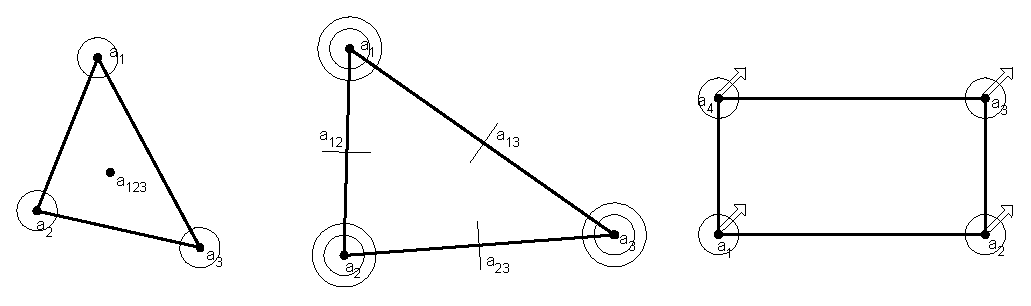
\includegraphics[width=\textwidth]{Hermite2D.eps}
\caption{\label{Hermite2D} Éléments finis d'Hermite triangulaire cubique, élément d'Argyris et élément rectangulaire $Q_3$}
\end{figure}


\medskip
\section{Traitement de plusieurs champs}\label{Sec-interf}

Dans ce qui précède, le lecteur aura noté que l'on interpole un seul
champ, en imposant ou non certaines régularités (dérivées partielles).

\medskip
Une question naturelle consiste à se demander comment traiter les
problèmes ayant plusieurs champs inconnus (cela à déjà été abordé,
et certaines stratégies on déjà été présentées: formulation mixte (Brezzi),\index[aut]{Brezzi (Franco), 1945-, Italien}
utilisation de multiplicateurs de Lagrange).\index[aut]{Lagrange (Joseph Louis, comte de -), 1736-1813, Italien}\index{Multiplicateurs de Lagrange}

On pourrait imaginer, si ces champs sont <<~dissociés~>> (sans lien les uns avec les
autres), de modéliser chaque champ séparément, i.e. de traiter un
problème par champ (avec pour chaque champ un choix de maillage et
d'élément qui lui est propre).

En fait, les problèmes à plusieurs champs ne concernent généralement
pas des champs indépendants.
Lorsque l'on  a plusieurs champs interdépendants, alors on dispose de relations
entre ces champs, qui doivent elles-aussi être satisfaites.

\medskip
Nous avons exposé au chapitre précédent pourquoi la mécanique reste un cas
compliqué. Cela provient de ce que les champs inconnus sont les déplacements,
déformations et contraintes.
De plus, le chapitre précédent a permis une illustration du choix d'un modèle,
même lorsque l'on ne recourt qu'à une théorie à un champ (déplacements).

\medskip
Nous ne construirons pas ici un élément à plusieurs champs, mais nous
allons donner une motivation pour le faire: celui du calcul des contraintes à
l'interface entre deux matériaux différents que nous supposerons parfaitement
collés.

Considérons donc le problème décrit à la figure \ref{interf}.
\begin{figure}[ht]
\centering
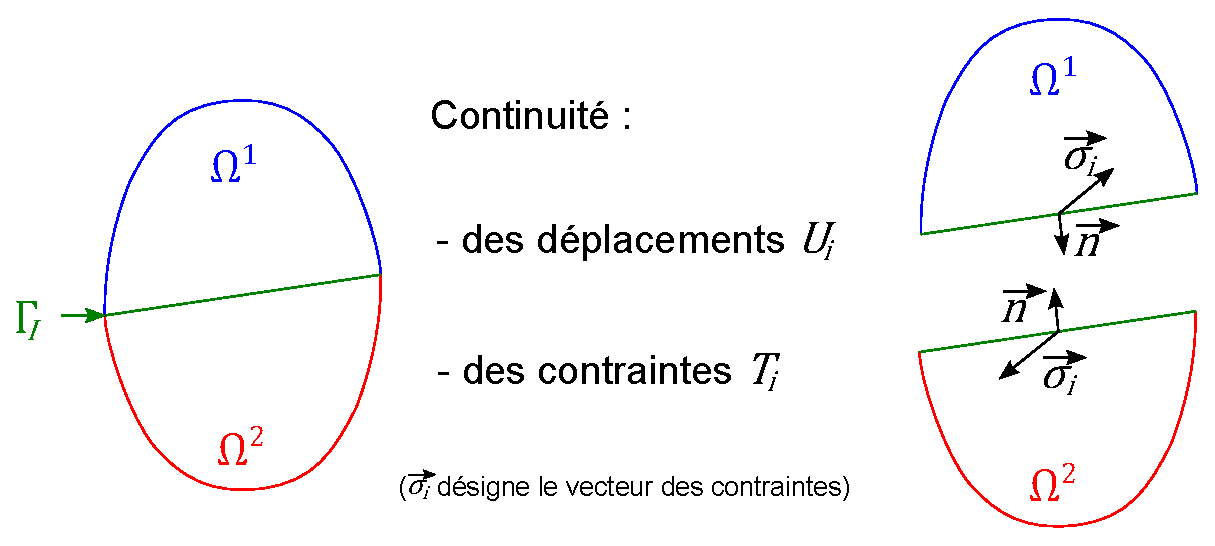
\includegraphics[height=50mm]{interface.eps}
\caption{\label{interf} Interface et continuités}
\end{figure}
Deux domaines $\Omega_1$ et $\Omega_2$, consittués chacun de leur
propre loi de comportement, ont une interface commune $\Gamma_I$.
On supposera que le champ de déplacement est continu le long de $\Gamma_I$.
La continuité de la composante normale du déplacement à l'interface traduit le
fait qu'il n'y a pas décollement entre les deux domaines; celle de la composante
tangentielle qu'il n'y a pas glissement entre eux.

On peut donc dire qu'en tout point de $\Gamma_I$ le déplacement est
continu, ce que l'on peut noter $u_i^1=u_i^2$.

\medskip
L'état d'équilibre des forces doit lui-aussi être vérifié le long de l'interface.
Cela implique que les composantes normales des contraintes doivent être également
continues le long de cette interface, i.e. que la trace du tenseur des contraintes doit
être continue le long de l'interface.
Par contre, les autres composantes peuvent (et doivent selon les cas) être
discontinues.

\bigskip
Plusieurs stratégies sont envisageables:
\begin{description}
\item[Post-traitement]\index{Post-traitement}

	Dans cette méthode, on effectue le calcul en déplacements, de manière classique.
	On obtient les contraintes de manière toute aussi classique, mais celles-ci
	n'ont évidemment pas les continuités et discontinuités souhaitées.

	On utilise une méthode de post-traitement qui va modifier le calcul des contraintes
	sur les éléments situés de part et d'autre de l'interface, par exemple
	en imposant la vérification des équations d'équilibre (voir par exemple
	la méthode de Reissner locale, qui applique la fonctionnelle de Reissner uniquement
	le long de l'interface).\index[aut]{Reissner (Max Erich, dit Eric), 1913-1996, Américain}
\item[Élément mixte]

	La fonctionnelle d'Hellinger-Reissner\index[aut]{Reissner (Max Erich, dit Eric), 1913-1996, Américain}\index[aut]{Hellinger} possède les champs de déplacement et de
	contrainte comme inconnues. Elle conduit à un système de type mixte
	(équation \eqref{Eq:SysMixte}) avec une matrice qui n'est plus définie-positive.

	Il s'en suit que ces deux champs sont continus, et notamment que toutes les
	composantes des contraintes le sont, ce qui ne satisfait pas les conditions
	d'équilibre.

	Si l'on souhaite utiliser ce type d'élément, il faudra par exemple, faire une
	condensation statique des composantes devant être discontinues, ou
	utiliser une méthode de post-traitement.
\item[Élément hybride]

	La fonctionnelle de Pian et Tong (mixte hybride)\index[aut]{Pian (Theodore H.H.), 1919-2009, Américain}\index[aut]{Tong (Pin), ? , Chinois}
	présentée précédemment
	a l'avantage de ne pas faire intervenir de dérivée. Elle conduit elle-aussi
	à un système de type mixte, mais la matrice de rigidité n'est même
	plus symétrique (dans une discrétisation <<~brutale~>>). On sait la retraiter.

	Toutes les composantes des contraintes sont là aussi continues, et il faudra appliquer les
	mêmes remèdes que ci-dessus.

	Notons qu'un avantage de cette formulation c'est qu'elle nécessite la matrice
	de souplesse $[S]$ au lieu de la matrice de Hooke $[H]$, ce qui permet de
	traiter le cas des matériaux incompressibles.\index{Loi de comportement!Hooke}\index{Loi de comportement!incompressible}\index[aut]{Hooke (Robert), 1635-1703, Anglais}
\item[Multiplicateurs de Lagrange]\index{Multiplicateurs de Lagrange}\index[aut]{Lagrange (Joseph Louis, comte de -), 1736-1813, Italien}
	
	D'une manière évidente, la continuité du champ de déplacements
	à l'interface $\li$ entre deux éléments $~^1$ et $~^2$ peut être
	imposée par l'ajout à al fonctionnelle de la condition:
	\begin{equation}   -\dint_{\li} \lambda_i(U_i^1-U_i^2)\ \dd\Gamma \end{equation}

	Cette condition est facile à écrire et facile à implémenter (mais on perd la
	définie-positivité de la matrice de rigidité).
	
	De plus, l'interprétation physique de ces multiplicateurs de Lagrange montre
	que ceux-ci sont égaux aux composantes normales des contraintes.
\end{description}
\medskip
Voilà quelques stratégies. D'autres peuvent exister, surtout si en plus on veut passer
sur des modèles poutre ou plaque.

Le but était de montrer que non seulement il est possible de développer de nombreux
éléments finis, mais que même à partir d'éléments existants, il est toujours
possible de construire une méthode numérique permettant d'obtenir les résultats
souhaités.

Les méthodes de post-traitement,\index{Post-traitement} que nous n'aborderons pas dans ce document,
sont très riches et permettent de faire beaucoup de choses.
Elles ont en outre l'avantage d'être parfois plus faciles à implémenter dans des
codes industriels que de nouveaux éléments.

\medskip
\section{Validation pratique et indicateurs d'erreur}\label{Sec-ValidEF}
Les tests numériques des éléments et au delà des codes de calcul sont indispensables.
Non seulement ils permettent de vérifier la satisfaction de critères de convergence
et d'évaluer la précision des éléments finis développés, ce qui peut être
réalisé par une analyse mathématique, mais ils permettent également de s'assurer
de la bonne programmation.
\medskip
Plusieurs types de tests peuvent et doivent être faits, sur plusieurs problèmes
types. Ces tests concernent aussi bien un seul élément, que plusieurs
(\textcolorblue{patch-test}),\index{Patch-Test} et même différents maillages.
\medskip
En mécanique, on distingue les cas listés dans le tableau~\ref{tab:Elem:test}.
\begin{table}[ht]\centering\footnotesize
\begin{tabular}{>{\raggedright\arraybackslash}p{25mm}|>{\raggedright\arraybackslash}p{25mm}|>{\raggedright\arraybackslash}p{35mm}|>{\raggedright\arraybackslash}p{35mm}}
\hline
Problème / solution de référence & Maillage & Vérification & Importance \\ \hline
Mouvement rigide et déformations constantes & 1 élément & base polynomiale complète / modes parasites & \multirow{2}{35mm}{convergence du modèle élément fini vers la solution théorique lorsque le nombre d'élément tend vers l'infini. Test particulièrement pour les non standard ou non conformes.} \\ \cline{1-3}
Mouvement rigide et déformations constantes & plusieurs éléments: patch-test cinématique\index{patch-test} ou mécanique & base complète, conformité, indépendance par rapport au maillage (vérification
de l'assemblage), absence de modes parasites & \\ \hline
Champ de déformations générales & différents maillages & précision et influence de la distorsion sur les déplacements et la contrante & qualité de l'élément par raport à d'autres éléments existants.\\
\hline
\end{tabular}\caption{Test de validation}\label{tab:Elem:test}
\end{table}

\medskip
\subsection{Modes rigides et parasites}
Le problème consiste à savoir si un élément fini, que l'on définira ici par sa matrice
$\MM{k}$, peut présenter l'état de déformation nulle ou d'énergie interne nulle (mode ou
mouvement de corps rigide).

\medskip
Une méthode consiste à déterminer le nombre de valeurs propres \textcolorred{nulles} de $\MM{k}$.
Ce nombre doit être égal au nombre de modes rigides: soit 3 en 2D (2 translations, 1 rotation),
6 en 3D, 1 en axisymétrique. On notera $m_r$ le nombre de modes rigides.
S'il y a plus de valeurs propres nulles que de modes rigides, alors c'est qu'il y a des
\textcolorblue{modes parasites} (à énergie nulle).
Ces modes parasites doivent disparaître après assemblage de plusieurs éléments
afin d'éviter que la matrice de rigidité soit singulière (d'où le test sur plusieurs éléments).
Le schéma d'intégration choisi pour la définition de l'élément (par exemple intégration
complète, réduite ou sélective) peut influer sur les modes parasites.
C'est pourquoi, il n'est pas toujours aussi simple de déterminer mathématiquement
ce facteur.

\medskip
Dans ce cas, il est possible d'introduire un champ de déplacement représentant le
mouvement rigide.
Pour chaque mode rigide $i$, le vecteur $\VV{u^i_n}$ associé à la matrice $\MM{k}$ doit
vérifier:
\begin{equation}\MM{k}\VV{u^i_n}=\VV{0}\end{equation}
Un mode rigide quelconque étant une combinaison linéaire des modes $\VV{u^i_n}$,
on construit un problème EF dans lequel on impose $m_r$ valeurs du vecteur $\VV{u^i_n}$
et on détermine numériquement les $n-m_r$ composantes (non imposées) de $\VV{u^i_n}$.
Celles-ci doivent être identiques aux valeurs théoriques associées au mode
rigide $i$. Si ce n'est pas le cas, c'est qu'il existe des modes rigides.
\medskip
\subsection{Modes associés aux déformations constantes}
Pour converger correctement l'élément doit également représenter
exactement l'état de déformations ou contraintes constantes (ou plus
généralement la représentation <<~constante~>> de tous les termes de la
forme variationnelle).

Dans un premier temps, on calcule les efforts nodaux correspondant à une contrainte fixée.

Dans un second temps, on introduit les efforts nodaux comme condition aux limites dans le modèle
élément fini et on vérifie si l'on retrouve bien l'état de contrainte initialement choisi.

\medskip
\subsection{Patch-tests}\index{Patch-Test}

Le domaine choisi doit posséder au moins un nœud à l'intérieur du domaine.

On définit un champ de déplacement conduisant à un état de déformation
désiré (constant ou non), que l'on introduit comme condition aux limites dans le modèle élément fini.

On vérifie qu'au point intérieur, l'état de déformation obtenu est bien celui
désiré.

\medskip
\subsection{Test de précision d'un élément}

On confronte le modèle élément fini à un ou des cas tests représentatifs de ce pour
quoi l'élément à été développé (élasticité tridimensionnelle,
bidimensionnelle, problème de torsion, problème avec concentrations locales de
déformations ou de contraintes, prise en compte des frontières courbes...).

Sur les composantes d'<<~intérêt~>>, on regardera s'il y a bien convergence
du modèle et sa vitesse de convergence en fonction du nombre d'éléments,
de la distorsion de ceux-ci...

\medskip
La <<~mesure~>> de l'écart peut demander une <<~jauge~>> particulière.
C'est ce que l'on appelle un \textcolorblue{estimateur d'erreur}.
Nous n'avons abordé jusqu'à présent que la mesure de l'erreur due à la
MEF elle-même, mais chaque problème particulier peut demander un
estimateur particulier.
Pour la mécanique, les estimateurs sont souvent liés à la qualité des
contraintes ou à des estimateurs d'énergie.

\medskip
Un \textcolorblue{indicateur local d'erreur} pourra par exemple être basé
sur l'écart entre les contraintes aux nœuds et aux frontières après
extrapolation des points d'intégration de chaque élément. On rappelle
que certaines contraintes doivent être nulles sur les frontières libres.

On trouve par exemple l'écart sur les contraintes équivalentes (selon un
sens à définir en fonction du type de matériau: par exemple von Mises\index[aut]{Mises (Richard Edler, von -), 1883-1953, Autrichien}
pour un matériau isotrope, Hill,\index[aut]{Hill (Rodney), 1921-2011, Anglais}
Tsaï-Hill,\index[aut]{Tsaï (Stephen W), ?-, Américain}
Tsaï-Wu...\index[aut]{Wu (Edward Ming-Chi), 1938-2009, Américain}
pour les matériaux anisotropes, les mousses, les os, les composites...);
l'écart sur la contrainte moyenne...

On peut également utiliser la densité d'énergie interne de
déformation sur chaque élément, l'idéal étant que tous les
éléments contribuent de manière identique à l'estimation de
l'énergie interne totale.

\medskip
Un \textcolorblue{indicateur global d'erreur} pourra être par exemple
la valeur de l'énergie potentielle totale. Plus sa valeur sera petite, meilleur
sera le modèle.

\medskip
On peut également vérifier que certaines équations d'équilibre sont vérifiées
à l'intérieur d'un élément ou le long d'une frontière entre éléments (par
exemple à l'interface entre deux domaines, un problème évoqué un peu avant
au paragraphe \ref{Sec-interf})...


\ifVersionAvecExemplesSepares\else
   \section{Exemple: quelques variations sur le thème des éléments unidimensionnels}

Dans ce paragraphe, nous appliquons ce que nous venons de voir sur quelques cas simples d'éléments unidimensionnels.

\medskipvm
\subsection{Élément de référence unidimensionnel linéaire à deux nœuds}\label{Sec-Elt1D2}

Considérons un segment reliant deux points dans l'espace. Ce segment est défini par un point courant dont les coordonnées sont le vecteur~$\VV{x}$. On peut paramétrer ce segment par le paramètre~$\xi \in [-1,1]$, et le vecteur position s'exprime par~$\LL{x}=\LL{x(\xi), y(\xi), z(\xi)}$.
\begin{figure}[ht]\centering\small
   \subfloat[Élément de référence]{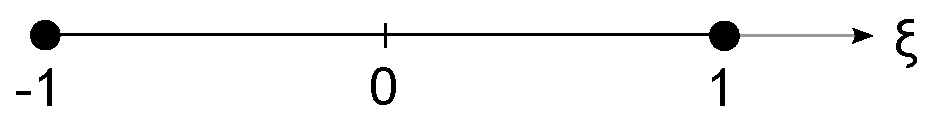
\includegraphics[width=60mm]{Elt1D-ref.eps}} \hspace{5em}
   \subfloat[Segment réel (3D)]{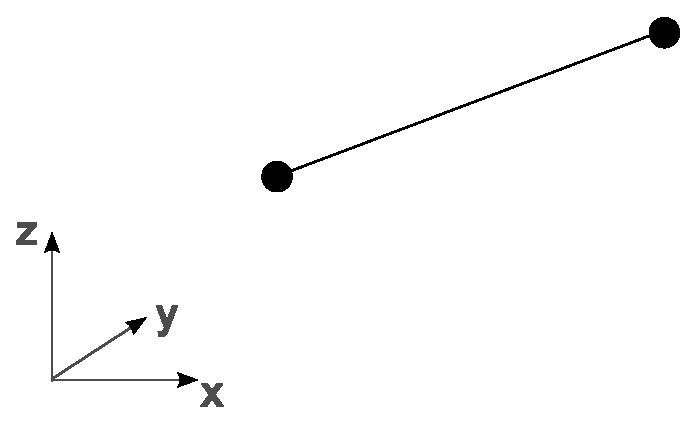
\includegraphics[width=40mm]{Elt1D-espace.eps}}
   \caption{Correspondance entre élément de référence et géométrie réelle}\label{fig-e1rr}
\end{figure}
\medskipvm
Cet élément (segment) est défini par ses seules extrémités. Nous avons donc deux nœuds de coordonnées~$\LLP{x_1, y_1, z_1}$ et~$\LLP{x_2, y_2, z_2}$.
\medskipvm
Un point courant de cet élément sera obtenu par interpolation linéaire entre les deux nœuds, paramétrée par~$\xi$. On Cherche cette interpolation sous la forme~$x(\xi)=\LL{N(\xi)}\VV{x_n}$, $y(\xi)=\LL{N(\xi)}\VV{y_n}$ et~$z(\xi)=\LL{N(\xi)}\VV{z_n}$, avec
$\LL{N(\xi)}=\LLL{N_1(\xi), N_2(\xi)}$ et~$N_1(\xi)=\frac12 (1-\xi)$, $N_2(\xi)=\frac12(1+\xi)$.
De manière plus «compacte», on peut écrire:
\begin{equation} N_i(\xi)=\frac12(1+\xi_i\xi), \qquad i=1,2, \quad \xi_i=\pm1 \quad (\text{et } \xi\in[-1,1]) \end{equation}
\medskipvm
Dans cette interpolation (comme dans toute interpolation), on a une relation entre~$\dd\VV{x}$ et $\dd\xi$. Notons~$\dd\VV{x} = \VV{a} \dd \xi$. Alors:
\begin{equation} \LL{a} = \LLL{x_{,\xi}, y_{,\xi}, z_{,\xi}} = \frac12 \LLL{x_{21}, y_{21}, z_{21}}\end{equation}
avec ici~$x_{21}=x_2-x_1$, $y_{21}=y_2-y_1$ et~$z_{21}=z_2-z_1$.
On voit ainsi comment passer d'une intégrale sur le segment réel à une intégrale sur l'élément de référence.

\medskipvm
De même, on peut chercher la relation entre~$\dd s=\dd\VV{x}\cdot\dd\VV{x}$. Nous notons $\dd s=m \dd \xi$. On a alors: 
\begin{equation}m=|\VV{a}| = \frac12 \sqrt{x_{21}^2+y_{21}^2+z_{21}^2} = \frac{L_e}2 \end{equation}
avec~$L_e$ la longueur de l'élément. On voit alors l'égalité des intégrations:
\begin{equation}\int_{L_e} \ldots \dd s = \int_{-1}^{+1}\ldots m \dd \xi\end{equation}

\medskipvm
Par ailleurs, on a la relation:
\begin{equation} \frac{\dd}{ \dd \xi} = \frac{\dd s}{ \dd \xi}\frac{\dd}{\dd s}=m\frac{\dd}{\dd s}\end{equation}

\medskip
\subsection{Rappels sur la jacobienne et le jacobien d'une transformation}\label{Sec-Jacob}\index{jacobien}\index{jacobienne}

Nous considérons une transformation de~$\RR^n$ dans~$\RR^m$ donnée par la fonction~$f$: 
$\left(x_1, \ldots, x_n \right) \mapsto \left(f_{y_1}, \ldots, f_{y_m} \right)$.
\medskipvm
La \textcolorblue{matrice jacobienne}\index{jacobienne} (d'après Carl Jacobi)\index[aut]{Jacobi (Carl Gustav Jakob), 1804-1851, Allemand} associée à~$f$ est définie par:
\begin{equation}
J_f = \MM*{\LL{\nabla f_{y_1}} \\ \vdots \\ \LL{\nabla f_{y_m}}}
\end{equation}
i.e., sous forme complètement développée la jacobienne de~$f$ s'écrit:
\begin{equation}
J_f = \MM*{\dfrac{\partial f_{y_1}}{\partial x_1} & \cdots & \dfrac{\partial f_{y_1}}{\partial x_n} \\ \vdots & \ddots & \vdots \\ \dfrac{\partial f_{y_m}}{\partial x_1} & \cdots & \dfrac{\partial f_{y_m}}{\partial x_n}}
\end{equation}
\medskipvm
Au voisinage d'un point~$M$, l'approximation linéaire de la fonction~$f$ est donnée par:
%\ifVersionDuDocEstVincent
\begin{equation} f\left(X\right) \approx f\left(M\right) + J_f\left(M\right) \overrightarrow{MX}\end{equation}
%\else
%\begin{equation} f\left(X\right) \approx f\left(M\right) + J_f\left(M\right) \mathbf{MX}%\end{equation}
%\fi
\medskipvm
La composée~$f\circ g$ de fonctions différentiables est différentiable, et sa matrice jacobienne s'obtient par la formule:
\begin{equation} J_{f \circ g}= \bigl( J_f \circ g \bigr) \cdot J_g\end{equation}
\medskipvm
Dans le cas où \textcolorred{$m = n$}, on appelle~$j_f$ le \textcolorblue{jacobien}\index{jacobien} de~$f$, 
défini comme le déterminant de sa matrice jacobienne: \index{jacobien}\index{jacobienne}
\begin{equation} j_f = \det\, \left(J_f \right) \end{equation}
Dire que le jacobien est non nul revient donc à dire que la matrice jacobienne est inversible.
\medskipvm
Si le jacobien\index{jacobien} est positif au point~$M$, l'orientation de l'espace est conservée au voisinage de ce point. À l'inverse, l'orientation est inversée si le jacobien est négatif.
\medskipvm
Le jacobien\index{jacobien} d'une composée de fonctions est le produit des jacobiens individuels.
\medskipvm
Le jacobien\index{jacobien} de la réciproque d'une fonction est l'inverse du jacobien de la fonction.
\medskipvm
\colorgris
Cette dernière propriété est liée au théorème d'inversion locale (qui peut être vu entre autre comme une extension du théorème des fonctions implicite en dimension supérieure à 1 dans le cas réel).
\medskipvm
Une fonction~$f$ de classe~$C^1$ est inversible au voisinage de~$M$ avec une réciproque~$f^{-1}$ de classe~$C^1$ si et seulement si son jacobien en~$M$ est non nul (théorème d'inversion locale). De plus, la matrice jacobienne de~$f^{-1}$ se déduit de l'inverse de la matrice jacobienne de~$f$ au moyen de la formule:\index{jacobien}\index{jacobienne}
\begin{equation}J_{f^{-1}} = \bigl( J_f \circ f^{-1} \bigr)^{-1}\end{equation}

\begin{theoreme}[Théorème d'inversion locale]\index{théorème!d'inversion locale}
Soit~$f$ une application de~$U$ dans~$F$, où~$U$ est un ouvert d'un espace de Banach réel et $F$ un espace de Banach et soit~$x$ un point de~$U$.

Si~$f$ est de classe~$C^p$, avec~$p$ un entier strictement positif et si la différentielle de~$f$ au point $x$ (définie au paragraphe \ref{Sec-Differentielle}) est un isomorphisme bicontinu, alors il existe un voisinage ouvert~$V$ de~$x$ et un voisinage ouvert $W$ de~$f(x)$ tels que~$f$ se restreigne en une bijection de~$V$ dans~$W$ dont la réciproque est de classe~$C^p$.
\end{theoreme}
\colorblack
\medskipvm
\textcolorgreen{Comme illustré au paragraphe précédent, le jacobien sert surtout pour effectuer des changement de variables dans le calculs des intégrales.}
\medskipvm
\begin{theoreme}[Théorème de changement de variables dans les intégrales multiples]\index{théorème!de changement de variables dans les intégrales multiples}
Soient~$U$ un ouvert de~$\RR^n$, $f$ une injection de classe~$C^1$ de~$U$ dans~$\RR^n$ et~$V=f(U)$.

Si~$g$ est une fonction mesurable de~$V$ dans~$\intfo{0}{+\infty}$, on a égalité des intégrales pour la mesure de Lebesgue sur~$\RR^n$:
\begin{equation}  \int_V g(y_1,\ldots,y_n)~\dd y_1\ldots\dd y_n = \int_U g\left(f\left(x_1,\ldots,x_n\right)\right) 
\left|\det J_f(x_1,\ldots,x_n)\right|~\dd x_1\ldots\dd x_n.
\end{equation}
\end{theoreme}
\medskipvm
\textcolorgreen{Si l'on considère un «petit» domaine, le volume de l'image de ce domaine par la fonction~$f$ sera celui du domaine de départ multiplié par la valeur absolue du jacobien.}\index{jacobien}

\medskip
\subsection{Éléments de référence unidimensionnels linéaires à~$n$ nœuds}

Il est possible de généraliser en considérant un segment ayant plusieurs nœuds intermédiaires comme indiqué sur la figure~\ref{fig:ex2:noeudint}.
\begin{figure}[ht]\centering
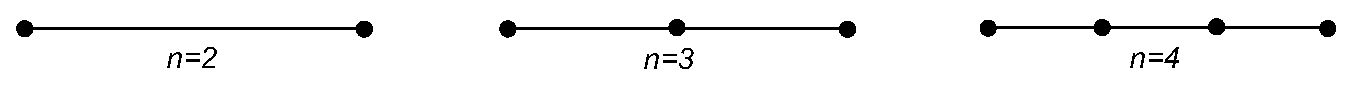
\includegraphics[width=140mm]{Elt1D-ex.eps}
\caption{Nœuds intermédiaires}\label{fig:ex2:noeudint}
\end{figure}
\medskipvm
Si l'on considère le cas général à~$n$ nœuds de la figure~\ref{fig:ex2:casgen}
\begin{figure}[ht]\centering
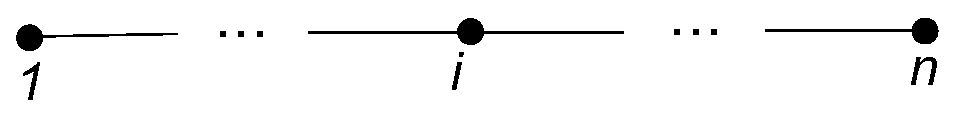
\includegraphics[width=60mm]{Elt1D-n.eps}
\caption{Cas général}\label{fig:ex2:casgen}
\end{figure}
alors il vient:
\begin{equation} N_i(\xi) = \prod_{r=1\atop r\ne i}^n \dfrac{\xi_r-\xi}{\xi_r-\xi_i} \end{equation}
\medskipvm
Si de plus, les~$n$ nœuds sont régulièrement espacés:
\begin{equation}\xi_i = -1+2\frac{i-1}{n-1} \qquad
N_i(\xi) = \prod_{r=1\atop r\ne i}^n \dfrac{(2r-n-1)-\xi(n-1)}{2(r-i)} \end{equation}

\medskip
\subsection{Élément de référence unidimensionnel infini}

Dans certains cas, il peut être nécessaire de prendre en compte des conditions aux limites situées à l'infini: problèmes de fondations, d'acoustique, de couplage fluide-structure.

Il est possible, comme aux paragraphes précédents, de proposer une transformation entre un élément de référence de longeur 2 et un élément réel infini, transformation illustrée sur la figure~\ref{fig:ex2:trans}.
\begin{figure}[ht]\centering
\begin{tabular}{cc}
\subfloat[Élément de référence]{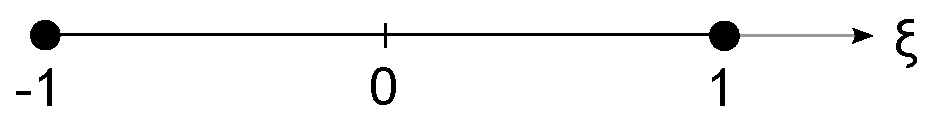
\includegraphics[width=65mm]{Elt1D-ref.eps}} \hspace{5em}
\subfloat[Élément réel (infini)]{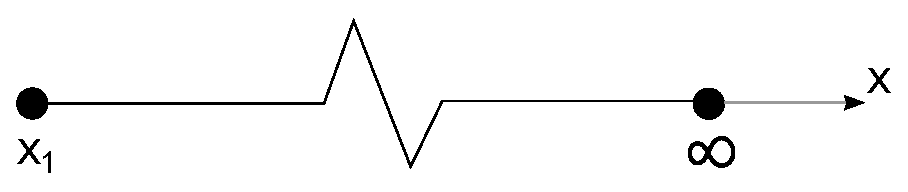
\includegraphics[width=65mm]{Elt1D-infty.eps}}
\end{tabular}\caption{Correspondance entre l'élément de référence et l'élément réel infini}\label{fig:ex2:trans}
\end{figure}
\medskipvm
Nous ne considèrerons que le cas de l'élément unidimensionnel linéaire à 2 nœuds dans ce paragraphe, mais on pourrait étudier le cas de l'élément linéaire unidimensionnel à~$n$ nœuds, ou des éléments bidimensionnels par exemple.
\medskipvm
Nous allons toujours avoir une interpolation de la fonction solution sous la forme:
\begin{equation} u =\frac{1-\xi}2 u_1 + \frac{1+\xi}2 u_2\end{equation}
car concrètement~$u_2$ est connu (et fini): c'est le «lieu» où l'on situe l'infini dans le modèle éléments finis.
\medskipvm
Par contre, l'interpolation du point courant sera donnée par:
\begin{equation}
x=x_1+\frac{1+\xi}{1-\xi}\alpha
\end{equation}
où~$\alpha$ est une constante.
\medskipvm
On aura également:
\begin{equation} u_{,x} = \frac{u_2-u_1}{4\alpha} (1-\xi)^2 \end{equation}

\medskip
\subsection{Élément fini de barre unidimensionnel}\label{Sec-barre1D}

On considère la barre de la figure~\ref{fig-barre}, de section~$A$, de longueur~$L$,  constituée d'un matériau homogène isotrope de module d'Young\index[aut]{Young (Thomas), 1773-1829, Anglais}\index{module d'Young} $E$ et densité~$\rho$ et soumise uniquement à son poids propre.
\begin{figure}[h!]
\centering
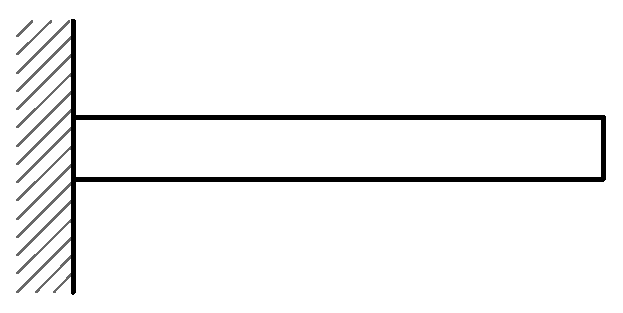
\includegraphics[width=40mm]{Elt1D-barre.eps}
\caption{Barre encastrée-libre}\label{fig-barre}
\end{figure}
On souhaite discrétiser ce problème à l'aide d'un élément unidimensionnel linéaire
tel que présenté au paragraphe~\ref{Sec-Elt1D2}.
\medskipvm
La forme variationnelle de ce problème d'élasticité linéaire unidimensionnel (théorie des poutres) est:
\begin{equation}
W=\dint_0^L EA v_{,x}u_{,x} \dd x - \dint_0^L \rho g A v = 0, \quad \forall v
\end{equation}
avec les conditions aux limites~$u(0)=0$ et~$v(0)=0$.
Cette forme variationnelle s'écrit pour l'élément (ou pour chaque élément si on en avait plusieurs):
\begin{equation}
W = \LL{v} \left( \MM{K}\VV{u} - \VV{f} \right)
\end{equation}
\medskipvm
Nous avons vu que la géométrie, représentée par un élément, est approximée par:
\begin{equation} x=\frac{1-\xi}2 x_1 + \frac{1+\xi}2 x_2, \quad \xi\in[-1;1] \end{equation}
La représentation de la fonction solution, est:
\begin{equation} u = \frac{1-\xi}2 u_1 + \frac{1+\xi}2 u_2, \quad \xi\in[-1;1] \end{equation}
\medskipvm
Nous obtenons la matrice de rigidité élémentaire:
\begin{equation} 
\MM{K} = \frac{2EA}L \MM*{1 & -1\\ -1& 1}
\end{equation}
et le vecteur des forces nodales élémentaires:
\begin{equation} 
\VV{f} = \rho g A \frac{L}4 \VV*{1 \\1}
\end{equation}
\medskipvm
En prenant en compte les conditions aux limites~$u_1=0$ et~$v_1=0$, l'expression~$W=0$ donne:
\begin{equation} u_2 = \frac{\rho g L^2}{8 E} \end{equation}
\medskipvm
La déformation est donnée par~$\varepsilon=u_{,x}=\LL{B}\VV{u_n}$ avec~$\LL{B}=\frac1L \LLL{-1, 1}$.
On obtient:
\begin{equation}
\varepsilon=\frac{\rho g L}{8 E}
\end{equation} 
Elle est constante sur l'élément. Quant à la contrainte, elle est obtenue par~$\sigma=E\varepsilon$, soit:
\begin{equation}\sigma=\frac{\rho g L}8\end{equation}
Elle est également constante sur l'élément.

\medskip
\subsection{Assemblage de trois éléments unidimensionnels linéaires à deux nœuds}\label{Sec-ass}

Poursuivons le cas de la poutre du paragraphe précédent, mais considérons une discrétisation de la barre à l'aide de trois éléments, comme montré sur la figure~\ref{fig-ex2ass}.
\begin{figure}[h!]\centering
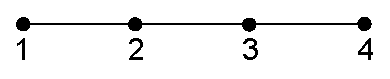
\includegraphics[width=60mm]{Elt1D-ass.eps}
\caption{Discrétisation de la barre en trois éléments}\label{fig-ex2ass}
\end{figure}
\medskipvm
Chaque élément~$e$ (de longueur~$L_e$) possède une matrice de rigidité élémentaire~$\MM{k_e}$ et un vecteur des forces nodales élémentaires~$\VV{f_e}$ définis par:
\begin{equation}\label{Eq-Ke}
\MM{K_e} = \frac{2EA}{L_e} \MM*{\begin{array}{cc} 1 & -1\\ -1& 1 \end{array}}
\qquad \text{ et } \qquad
\VV{f_e} = \rho g A \frac{L_e}4 \VV*{\begin{array}{c} 1 \\1 \end{array}}
\end{equation}
\medskipvm
Les variables nodales sont~$\LL{q}=\LL{u_1, u_2, u_3, u_4}$. Les matrices élémentaires,
issues de l'équation~(\ref{Eq-Ke}), s'écrivent en fonction de ces variables nodales:
\begin{equation*}
\MM{K}_1 = \frac{2EA}{L_1} \MM*{1 & -1 & 0 & 0\\ -1& 1 & 0 & 0\\ 0&0&0&0\\0&0&0&0}
\quad
\MM{K}_2 = \frac{2EA}{L_2} \MM*{0&0&0&0\\ 0& 1 & -1 & 0\\ 0 & -1& 1& 0\\0&0&0&0}
\quad
\MM{K}_3 = \frac{2EA}{L_3} \MM*{0&0&0&0\\0&0&0&0\\0& 0& 1 & -1\\ 0&0 & -1& 1}
\end{equation*}
et les forces nodales, quant à elles, s'expriment sous la forme:
\begin{equation*}
\VV{f_1} = \rho g A \frac{L_1}4 \VV*{1 \\1\\0\\0}
\quad
\VV{f_2} = \rho g A \frac{L_2}4 \VV*{0\\1 \\1\\0}
\quad
\VV{f_3} = \rho g A \frac{L_3}4 \VV*{0\\0\\1 \\1}
\end{equation*}
\medskipvm
L'\textcolorblue{assemblage} permettant de constituer le système complet est simplement obtenu par:
\begin{equation} \MM{K}=\MM{K}_1+\MM{K}_2+\MM{K}_3 \qquad \text{ et } \qquad \VV{F}=\VV{f_1}+\VV{f_2}+\VV{f_3} \end{equation}
\medskipvm
On résout alors~$\MM{K}\VV{q}=\VV{F}$ avec la condition aux limites~$u_1=0$.

\medskip
\begin{remarque}
La matrice~$\MM{K}$ obtenue sur cet exemple a un \textcolorblue{caractère bande} (la matrice est vide en dehors d'une zone centrée sur la diagonale). Ceci est dû à la numérotation des nœuds. Une autre numérotation pourrait faire perdre ce caractère important (stockage et résolution).
C'est pourquoi les programmes éléments finis peuvent comporter une étape de renumémoration automatique des nœuds.
\end{remarque}

\medskip
\subsection{Élément de barre unidimensionnel de type Hermite (élément subparamétrique)}\index[aut]{Hermite (Charles), 1822-1901, Français}\index{élément fini!d'Hermite}

En restant encore sur notre élément linéaire unidimensionnel, nous allons voir comment ajouter des contraintes sur les dérivées aux nœuds, comme illustré à la figure~\ref{fig-ex2Her}.
\begin{figure}[h!]\centering
\subfloat[Élément de référence]{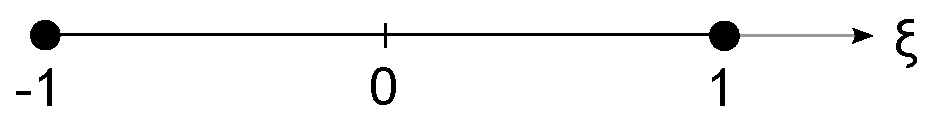
\includegraphics[width=60mm]{Elt1D-ref.eps}} \hspace{5em}
\subfloat[Segment réel (2 nœuds, 4ddl)]{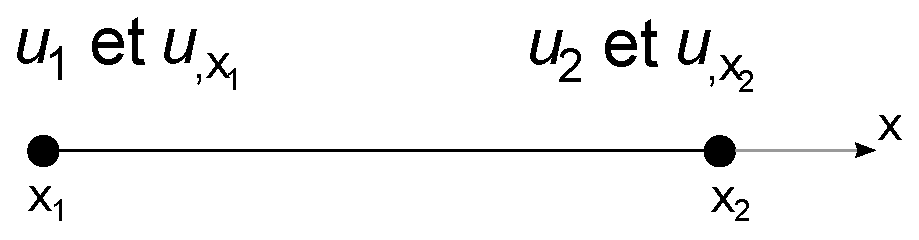
\includegraphics[width=60mm]{Elt1D-hermite.eps}}
\caption{Élément de barre unidimensionnel de type Hermite}\label{fig-ex2Her}
\end{figure}
\medskipvm
La géométrie est encore une fois approximée par:
\begin{equation} x=\frac{1-\xi}2 x_1 + \frac{1+\xi}2 x_2, \quad \xi\in[-1;1] \end{equation}
\medskipvm
Mais cette fois, l'approximation de la fonction solution est voulue sous la forme:
\begin{equation}
u = \LLL{N_1, N_2, N_3, N_4}\VV{u_n} \qquad \text{ avec les ddl } \qquad
\LL{u_n}=\LLL{u_1, u_{,x_1}, u_2, u_{,x_2}} 
\end{equation}
\medskipvm
Les fonctions~$N_i$ choisies sont des fonctions cubiques de type Hermite assurant une continuité de~$u$ et~$u_{,x}$ aux nœuds 1 et 2. On a:
\begin{equation}
N_1=\frac14(1-\xi)^2(2+\xi); \qquad
N_2=\frac{L}8(\xi^2-1)(1-\xi); \qquad
N_3=\frac14(1+\xi)^2(2-\xi); \qquad
N_2=\frac{L}8(\xi^2-1)(1+\xi)
\end{equation}
\medskipvm
Le champ~$u_{,x}$, qui est la déformation~$\varepsilon$, est donné par~$\varepsilon=\LL{B}\{u_n\}$ avec:
\begin{equation} \LL{B}=\LLL{\frac3{2L}(\xi^2-1), \quad \frac14(3\xi^2-2\xi-1), \quad \frac3{2L}(1-\xi^2), \quad
\frac14(3\xi^2+2\xi-1)}\end{equation}
\medskipvm
La contrainte, dans le cas où le coefficient d'élasticité~$H$ est constant est donnée par:
\begin{equation}\sigma_x=H \LL{B}\VV{u_n}\end{equation}

\medskip
\subsection{Élément mixte unidimensionnel}

Continuons avec notre élément de référence linéaire unidimensionnel. Cette fois-ci nous souhaitons le mettre en relation avec un segment réel dont les inconnues nodales sont les déplacements $u_1$ et~$u_2$, mais qui possède en plus une approximation constante de la contrainte par élément, comme montré sur la figure~\ref{fig-ex2mixte}.
\begin{figure}[ht]\centering
\subfloat[Élément de référence]{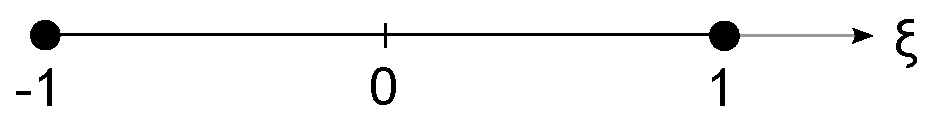
\includegraphics[width=60mm]{Elt1D-ref.eps}} \hspace{5 em}
\subfloat[Élément réel]{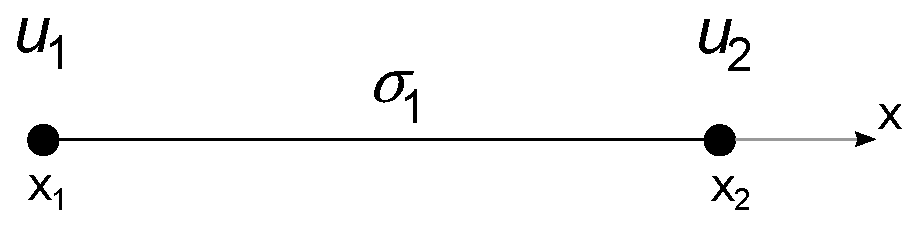
\includegraphics[width=60mm]{Elt1D-mixte.eps}}
\caption{Élément mixte unidimensionnel}\label{fig-ex2mixte}
\end{figure}
\medskipvm
Nous cherchons donc une approximation~$C^0$ du déplacement et~$C^{-1}$ de la
contrainte.
\medskipvm
Pour la géométrie, nous avons une fois encore:
\begin{equation} x=\frac{1-\xi}2 x_1 + \frac{1+\xi}2 x_2, \quad \xi\in[-1;1] \end{equation}
\medskipvm
Pour la contrainte, nous avons:
\begin{equation} \sigma_x(x)=\sigma_1 \text{ (constante)} \end{equation}
\medskipvm
La fonctionnelle d'Hellinger-Reissner sous sa deuxième forme (ou fonctionnelle mixte), donnée dans sa formulation générale par l'équation~(\ref{Eq-HR2}),\index[aut]{Reissner (Max Erich, dit Eric), 1913-1996, Américain}\index[aut]{Hellinger (Ernst David), 1883-1950, Allemand}\index{fonctionnelle!d'Hellinger-Reissner}\index{fonctionnelle!mixte} s'écrit, dans le cas de l'élasticité linéaire unidimensionnelle:
\begin{equation}
W=\dint_0^L A\left(-\sigma_x^*\frac1H\sigma_x+\sigma_x^*u_{,x}+v_{,x}\sigma_x\right) \dd x
-\dint_0^L Avf_x \dd x - (v f_S)_{S_f} = 0\qquad \forall v,\sigma^*
\end{equation}
avec les conditions aux limites~$u=\overline{u}$ et~$u^*=0$ sur~$S_u$.
\medskipvm
De manière discrétisée, il vient:
\begin{equation}
W = \LLL{v_1, v_2, \sigma_1^*}\left(
\MM*{\mO & \VV{b}\\ ~\\ \LL{b} & -a}
\VV*{u_1\\u_2\\ \sigma_1}
- \VV*{\VV{f_n}\\~\\ \sigma_1}
\right)\end{equation}
avec:
\begin{equation}
\VV{b}=\dint_0^L \frac{A}L \VV*{-1\\1}; \qquad
a=\dint_0^L \frac{A}H \dd x; \qquad
\VV{f_n} = \dint_{-1}^{+1} A \VV*{N_1\\N_2} \frac{L}2 f_x \dd\xi =
 A f_x \frac{L}2 \VV*{1\\1}
\end{equation}
\medskipvm
On pourrait s'arrêter là avec le système précédent à résoudre. Toutefois, $\sigma_1$ est une variable locale sans couplage avec les autres éléments. On peut donc l'exprimer en fonction des autres degrés de liberté de l'élément~$u_1$ et~$u_2$. La dernière ligne du système donne:
$\sigma_1^*=\left(\LL{b}\VV{u_n}-a\sigma_1\right)=0$, $\forall \sigma_1^*$,
d'où:
\begin{equation} \sigma_1 = \frac1a \LL{b}\VV{u_n} \end{equation}
\medskipvm
Le système devient alors:
\begin{equation} W=\LL{v_n}\left( \VV{b}\sigma_1 -\VV{f_n}\right) =
\LL{v_n} \left( \MM{K}\VV{u_n}-\VV{f_n}\right) \end{equation}
avec:
\begin{equation} \MM{K}=\VV{b}\frac1a\LL{b} \end{equation}
Dans le cas où~$H$ est constant, la matrice de rigidité obtenue est identique à celle du modèle en déplacements du paragraphe~\ref{Sec-barre1D}.
% élts 1D
   \section{Sur les déplacements imposés}\label{Ch-DispLag}% et les multiplicateurs de Lagrange}

\medskip
\subsection{Problème considéré}

Nous repartons de l'élément de barre 1D défini au paragraphe~\ref{Sec-barre1D}, et nous rappelons que la matrice de rigidité élémentaire et le vecteur des forces nodales élémentaires sont:
\begin{equation} \MM{K} = \frac{2EA}L \MM*{1 & -1\\ -1& 1} %\end{equation}
\qquad \text{ et } \qquad
\VV{f} = \rho g A \frac{L}4 \VV*{1 \\1} \end{equation}
\medskipvm
L'assemblage de trois éléments, décrit au pagraphe~\ref{Sec-ass}, conduit à:
\begin{equation} \MM{K}=\MM{K_1}+\MM{K_2}+\MM{K_3} \qquad \text{ et } \qquad \VV{F}=\VV{f_1}+\VV{f_2}+\VV{f_3} \end{equation}
\medskipvm
On traitera le cas où les trois éléments ont la même longueurs ($L_1=L_2=L_3=L$) et où seul le nœud 4 est soumis à une force.
%\medskip
%Dans ce cas, on obtient les matrices élémentaires:
%\begin{equation}
%[k_1] = \frac{2EA}{L} \left[ \begin{array}{cccc} 1 & -1 & 0 & 0\\ -1& 1 & 0 & 0\\ 0&0&0&0\\0&0&0&0 \end{array}\right]
%\quad
%[k_2] = \frac{2EA}{L} \left[ \begin{array}{cccc}0&0&0&0\\ 0& 1 & -1 & 0\\ 0 & -1& 1& 0\\0&0&0&0 \end{array}\right]
%\quad
%[k_3] = \frac{2EA}{L} \left[ \begin{array}{cccc}0&0&0&0\\0&0&0&0\\0& 0& 1 & -1\\ 0&0 & -1& 1\end{array}\right]
%\end{equation}
%et les forces nodales:
%\begin{equation}
%\{f_1\} = \{f_2\} = \left\{ \begin{array}{c} 0\\0 \\0\\0 \end{array}\right\}
%\quad
%\{f_3\} = \rho g A \frac{L}4 \left\{ \begin{array}{c} 0\\0\\0 \\1 \end{array}\right\}
%\end{equation}
%
%\medskip
%On s'intéresse à la résolution du système~$[K]\{q\}=\{F\}$ avec les conditions aux limites~$u_1=0$.
%Explicitement, on s'intéresse donc à la résolution du système:
%\medskip
On obtient alors un système de type~$\MM{K}\VV{q}=\VV{F}$ à résoudre, avec la condition aux limites~$u_1=0$, qui s'écrit explicitement dans ce cas:
\begin{equation}
\MM*{1 & -1 & 0 & 0 \\ -1 & 2 & -1 & 0 \\ 0 & -1 & 2 & -1\\ 0&0&-1&1}
\VV*{u_1\\u_2\\u_3\\u_4}
=
\VV*{0\\0\\0\\F'}
\end{equation}
(avec~$F'=\rho g L^2/(8E)$).

\medskip
\subsection{Retour sur la résolution de systèmes linéaires}

Soit à résoudre un système linéaire de type:
\begin{equation}\label{Eq-lin} \MM{A}\VV{x}=\VV{b} \end{equation}
Ce système peut être réécrit par blocs sous la forme:
\begin{equation} 
\MM*{A_{11} & A_{12}\\ A_{21} & A_{22}}
\VV*{x_1 \\ x_2} =
\VV*{b_1\\ b_2}
\end{equation}
\medskipvm
Si~$A_{11}$ est inversible, alors on peut écrire la première ligne:
\begin{equation}
x_1 = A_{11}^{-1}\left( b_1-A_{12}x_2 \right)
\end{equation}
ce qui donne, dans la deuxième ligne:
\begin{equation}
A_{22} - A_{21}A_{11}^{-1}A_{12}x_2 = b_2 - A_{21}A_{11}^{-1}b_1
\quad \text{ que l'on note: }
S x_2=c
\end{equation}
\textcolorblue{La matrice~$S$ est appelée complément de Schur}\index{complément de Schur}\index[aut]{Schur (Issai), 1875-1941, Russe} (présenté au paragraphe~\ref{Sec-Schur}), ou matrice condensée sur les degrés de liberté~$x_2$. Ce calcul est également identique à celui présenté à propos de la condensation statique au paragraphe~\ref{Sec-condens}. Dans ce cas, la matrice~$S$ est la matrice de rigidité du super-élément considéré.

\medskip
Le système initial (\ref{Eq-lin}) est équivalent à:
\begin{equation}\label{Eq-Sch1}
\MM*{A_{11} & A_{12}\\ \mO & S}
\VV*{x_1\\ x_2} =
\VV*{b_1\\ c}
\end{equation}
qui peut être réécrit:
\begin{equation}
\MM*{I & \mO{} \\ A_{21}A_{11}^{-1} & I}
\MM*{A_{11} & A_{12}\\ \mO{} & S}
\VV*{x_1\\ x_2} =
\MM*{I & \mO{} \\ A_{21}A_{11}^{-1} & I}
\VV*{b_1\\ c}
\end{equation}

\medskip
\subsection{Complément de Schur et déplacements imposés}\index{complément de Schur}\index[aut]{Schur (Issai), 1875-1941, Russe}

Nous cherchons toujours à résoudre notre système:
\begin{equation}\MM{K}\VV{q}=\VV{f}\end{equation}

\medskip
Considérons la matrice~$\MM{D}$, \textcolorblue{matrice booléenne}, permettant d'extraire de l'ensemble des inconnues nodales~$\VV{q}$ le sous-ensemble~$\VV{q_2}=\MM{D}\VV{q}$ sur lesquels portent les conditions de déplacements imposés~$\VV{q_d}$ \textcolorred{(ici on traite le cas général, i.e. les déplacements imposés peuvent être nuls ou non)}. La matrice \textcolorblue{$\MM{D}$ n'est pas rectangulaire}: si on souhaite imposer~$d$ déplacements parmi les~$n$ degrés de liberté du système, alors~$\MM{D}$ est de dimension~$d\times n$, et donc~$\VV{q_2}$ est bien un vecteur à~$d$ composantes, comme~$\VV{u_d}$.

\medskip
Le système~$\MM{K}\VV{q}=\VV{F}$ peut alors s'écrire, par blocs, en utilisant le complément de Schur (\ref{Eq-Sch1}) sous une forme triangulaire d'où l'on tire le sous-système correspondant aux déplacements non imposés:
\begin{equation}
\MM{K_{11}}\VV{q_1} = \VV{f_1} - \MM{K_{12}}\VV{u_d}
\end{equation}
\medskipvm
Ce système est \textcolorblue{réduit}, i.e. possède moins d'inconnues que le problème initial, mais il est nécessaire de modifier le chargement extérieur.

Son inconvénient est qu'il est nécessaire d'effectuer un \textcolorred{tri explicite} au sein des degrés de liberté, ce qui a pour conséquence de «remplir» le terme~$\MM{K_{12}}$, et par suite peut générer un surcoût de calcul lorsque le nombre de degrés de liberté bloqués est grand.

C'est ainsi que procède le code \abaqus pour imposer les déplacements.

\medskip
\subsection{Multiplicateurs de Lagrange et déplacements imposés}\index{multiplicateurs de Lagrange}\index[aut]{Lagrange (Joseph Louis, comte de -), 1736-1813, Italien}\label{Sec-cast}

Une autre technique, pour imposer des déplacements, consiste à utiliser les multiplicateurs de Lagrange:\index{multiplicateurs de Lagrange}\index[aut]{Lagrange (Joseph Louis, comte de -), 1736-1813, Italien} les contraintes sont relaxées, puis réintroduites via des multiplicateurs de Lagrange.

Dans ce cas, il n'est plus nécessaire de séparer explicitement les degrés de liberté, mais \textcolorred{la taille du problème augmente} puisqu'il faut lui adjoindre les multiplicateurs.

Le système à résoudre s'écrit très simplement:
\begin{equation}\label{Eq-Lag1}
\MM*{\MM{K} & -\MM{D}^T\\ -\MM{D} & \mO{}}
\VV*{q\\ \lambda} =
\MM*{A}
\VV*{q\\ \lambda} =
\VV*{F\\ -u_d}
\end{equation}
Il est intéressant de remarquer que la première ligne montre que \textcolorblue{les multiplicateurs de Lagrange sont bien les réactions aux appuis}.\index{multiplicateurs de Lagrange}\index[aut]{Lagrange (Joseph Louis, comte de -), 1736-1813, Italien}

Par contre, la matrice du système (\ref{Eq-Lag1}), $\MM{A}$, si elle reste bien symétrique, \textcolorred{n'est plus définie positive}. Elle possède des valeurs propres négatives.
%%%%%%%%%%%%%%%%%%%
\medskipvm
Toutefois, on dispose du résultat suivant:

\begin{theoreme}
si~$\MM{K}$ est symétrique définie positive, alors:
\begin{equation}
\MM{A} \text{ inversible } \Longleftrightarrow \MM{D} \text{ injective } \Longleftrightarrow \ker \MM{D} = \emptyset
\end{equation}
\end{theoreme}
ce qui correspond aux cas où toutes les liaisons sont indépendantes.

\bigskipvm
Afin de ne pas détruire la structure bande de~$\MM{K}$ (ce que ferait une factorisation de Gauß),\index[aut]{Gauß (Johann Carl Friedrich), 1777-1855, Allemand} et d'éviter des pivotages (que ferait une factorisation de Crout, i.e.~$\MM{LDL}^T$), on peut développer une autre technique, dite \textcolorblue{technique de double multiplicateur}, qui est celle employée dans \castem:\index{multiplicateurs de Lagrange}\index[aut]{Lagrange (Joseph Louis, comte de -), 1736-1813, Italien}
\begin{equation}
\left\{\begin{aligned}
&\MM{K}\VV{q} = \VV{F} - \MMT{D}\left(\VV{\lambda_1} - \VV{\lambda_2}\right) \\
&\VV{\lambda_1} = \VV{\lambda_2} \\ 
&\MM{D}\VV{q} = \VV{u_d}
\end{aligned}\right.
\end{equation}
\textcolorred{L'inconvénient reste l'augmentation de la taille du système lorsque l'on a de nombreux blocages.}

\medskip
\subsection{Actions extérieures et déplacements imposés}

L'interprétation physique des multiplicateurs de Lagrange conduit naturellement à une autre méthode: il est possible de considérer un déplacement imposé comme une action extérieure, par exemple comme la réaction d'un ressort ayant une raideur~$k$ très grande et un déplacement imposé à sa base.

\medskip
On se retrouve alors avec un système du type:
\begin{equation}
\left(\MM{K} + \MMT{D}k\MM{D}\right) \VV{q} = \VV{F} + \MMT{D}k\MM{D}\VV{u_d}
\end{equation}
dans lequel on n'a fait qu'ajouter des termes à la matrice de rigidité sur les degrés de liberté correspondant à ces déplacements et au vecteur des forces généralisées sur les efforts duaux.

\medskip
\textcolorred{Le problème réside dans le choix de la valeur de~$k$}: trop petite, la condition est mal imposée; trop grande, le système devient très mal conditionné, voire numériquement singulier.

\medskip
\subsection{Retour sur notre exemple}

Nous devons toujours résoudre:
\begin{equation}
\MM*{1 & -1 & 0 & 0 \\ -1 & 2 & -1 & 0 \\ 0 & -1 & 2 & -1\\ 0&0&-1&1}
\VV*{u_1\\u_2\\u_3\\u_4}
=
\VV*{0\\0\\0\\F'}
\end{equation}
avec la condition aux limites~$u_1=0$.
\medskipvm
Tout d'abord, on pourra essayer de résoudre sans introduire de conditions aux limites afin de voir que le système est alors singulier. On obtient~$u_1=u_2=u_3=u_4$ et~$F'=0$.
\medskipvm
La méthode la plus rudimentaire consiste à prendre en compte directement et explicitement la condition aux limites. On supprime donc du système matriciel la ligne et la colonne correspondant à~$u_1$, et on résout:
\begin{equation}\label{Eq-Base}
u_1=0 \text{ et }
\MM*{2 & -1 & 0 \\ -1 & 2 & -1\\ 0&-1&1}
\VV*{u_2\\u_3\\u_4}
=
\VV*{0\\0\\F'}
\qquad \text{ d'où: } 
\left\{\begin{aligned} &u_1=0 \\ &u_2=F' \\ &u_3=2F' \\ &u_4=3F' \end{aligned}\right.
\end{equation}
\medskipvm
Séparons maintenant les déplacements imposés des autres degrés de liberté, par une matrice booléenne~$\MM{D}$:
$\MM{D}$ est une matrice~$1\times 4$, et seul le terme~$D_{11}=1$ est non nul:~$\VV{q_2}=\MM{D}\VV{q}=\VV{u_1}$,
et le déplacement imposé est~$\VV{u_d}=\VV{0}$.

Le système s'écrit:
\begin{equation}
\MM*{K_{11} & K_{12}\\ K_{21} & K_{22}}
\VV*{q_1\\ q_2} =
\VV*{f_1\\ f_2}
\end{equation}
avec:
\begin{equation*}
%\left[\begin{array}{cc} K_{11} & K_{12}\\ K_{21} & K_{22} \end{array} \right]
%\left\{\begin{array}{c} q_1\\ q_2 \end{array} \right\} =
%\left\{\begin{array}{c} f_1\\ f_2 \end{array} \right\} 
%\text{ i.e. }
\MM*{%
\MM{K}_{11}=\MM*{2 & -1 & 0 \\ -1 & 2 & -1\\ 0 & -1 & 1} &
\MM{K}_{12}=\MM*{-1 \\ 0\\ 0}\\
\MM{K}_{21}=\MM*{-1 & 0 & 0} &
% \left[ \begin{array}{c} 1 \end{array} \right]
\MM{K}_{22} =\MM*{1}
}
\VV*{\VV{q}_1=\VV*{u_2\\u_3\\u_4}\\
\VV{q}_2 =\VV*{u_1}}
=
\VV*{\VV{f}_1 =\VV*{0\\0\\F'}\\ 
\VV{f}_2=\VV*{u_d=0}}
\end{equation*}
\medskipvm
Par la méthode du complément de Schur, on est encore ramené à la résolution du système (\ref{Eq-Base}). On pourra s'amuser à calculer~$\MM{K}_{11}^{-1}$, $\MM{S}$...
%$[K_{11}]^{-1} = \left[\begin{array}{ccc} 1&1&1 \\ 1&2&2\\ 1&2&3 \end{array} \right]$
\medskipvm
Par la méthode des multiplicateurs de Lagrange, on obtient le système:
\begin{equation}
%\MM{\begin{array}{ccccc} 1& -1 & 0 & 0 & -1 \\ -1 & 2 & -1 & 0 & 0 \\ 0 & -1 & 2 & -1 & 0\\ 0&0&-1&1& 0 \\ -1&0&0&0&0 \end{array}}
\MM*{1& -1 & 0 & 0 & -1 \\ -1 & 2 & -1 & 0 & 0 \\ 0 & -1 & 2 & -1 & 0\\ 0&0&-1&1& 0 \\ -1&0&0&0&0}
\VV*{u_1\\u_2\\u_3\\u_4\\ \lambda}
=
\VV*{0\\0\\0\\F' \\ u_d=0}
\qquad \text{ d'où: } 
\left\{\begin{array}{l} u_1=0 \\ u_2=F' \\ u_3=2F' \\ u_4=3F' \\ \lambda = -F' \end{array}\right.
\end{equation}
\medskipvm
Par la technique du double multiplicateur, on obtient le système:
\begin{equation}
\MM*{1 & -1 & 0 & 0 & 1&-1 \\ -1 & 2 & -1 & 0 & 0&0 \\ 0 & -1 & 2 & -1 & 0&0\\ 0&0&-1&1& 0&0 \\ 1&0&0&0&0&0}
\VV*{u_1\\u_2\\u_3\\u_4\\ \lambda_1 \\ \lambda_2}
=
\VV*{0\\0\\0\\F' \\ 0 \\ u_d=0}
\qquad \text{ d'où: } 
\left\{\begin{array}{l} u_1=0 \\ u_2=F' \\ u_3=2F' \\ u_4=3F' \\ \lambda_1 = -F' \\ \lambda_2 = -F' \end{array}\right.
\end{equation}
\medskipvm
En considérant une action extérieure, on obtient le système:
\begin{equation}
\MM*{1+k & -1 & 0 & 0 \\ -1 & 2 & -1 & 0 \\ 0 & -1 & 2 & -1\\ 0&0&-1&1}
\VV*{u_1\\u_2\\u_3\\u_4}
=
\VV*{0+k\cdot u_d = 0\\0\\0\\F'}
\qquad \text{ d'où: } 
\left\{\begin{array}{l} u_1=0 \\ u_2=F' \\ u_3=2F' \\ u_4=3F' \end{array}\right.
\end{equation}

\medskip
Dans tous les exemples présentés, nous avons résolu les systèmes à la main, ce qui masque d'éventuels problèmes numériques (notamment dans le dernier cas).

\medskip
\subsection{Relations linéaires entre ddl}

Cette situation se présente par exemple lors de la prise en compte de conditions de symétrie, de conditions aux limites périodiques... Il s'agit à chaque fois de conditions de type:
\begin{equation}
\MM{D}\VV{q} = \VV{u_d}
\end{equation}
où~$\MM{D}$ n'est plus forcément booléenne.

\medskip
Nous allons l'appliquer ici, à titre d'exemple simple, au cas où la poutre considérée est maintenant constituée de deux poutres, que l'on va «coller» par une telle relation.
\begin{figure}[ht]
\centering
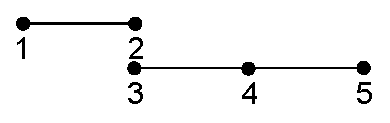
\includegraphics[width=60mm]{Elt1D-ass2.eps}
\end{figure}
La poutre est constituée de la poutre~$1-2$ et de la poutre~$3-4-5$, les points~$2$ et~$3$ étant astreints à rester collés ensembles.
\medskipvm
En ajoutant la relation~$u_2=u_3$ par l'intermédiaire d'un multiplicateur de Lagrange\index{multiplicateurs de Lagrange}\index[aut]{Lagrange (Joseph Louis, comte de -), 1736-1813, Italien}, c'est-à-dire en ajoutant le terme~$\lambda_1(u_2-u_3$), on obtient le système:
\begin{equation}
\MM*{1&-1&0&0&0&0 \\ -1&1&0&0&0&1 \\ 0&0&1&-1&0&-1\\ 0&0&-1&2&-1&0\\ 0&0&0&-1&1&0 \\ 0&1&-1&0&0&0}
\VV*{u_1\\u_2\\u_3\\u_4\\ u_5\\ \lambda_1}
=
\VV*{0\\0\\0\\F' \\ 0 \\ u_d=0}
\end{equation}
auquel il faut également ajouter la condition aux limites~$u_1$=0.

Si cette condition aux limites est imposée par un multiplicateur de Lagrange~$\lambda_2$, alors finalement, il faut résoudre:
\begin{equation}
\MM*{1&-1&0&0&0&0&-1 \\ -1&1&0&0&0&1&0 \\ 0&0&1&-1&0&-1&0\\ 
0&0&-1&2&-1&0&0\\ 0&0&0&-1&1&0&0 \\ 0&1&-1&0&0&0&0 \\ 1&0&0&0&0&0&0}
\VV*{u_1\\u_2\\u_3\\u_4\\ u_5\\ \lambda_1 \\ \lambda_2}
=
\VV*{0\\0\\0\\F' \\ 0 \\ 0 \\ 0}
\qquad \text{ d'où: } 
\left\{\begin{array}{l} u_1=0 \\ u_2=F' \\ u_3=F' \\ u_4=2F' \\ u_5=3F' \\ \lambda_1 = -F' \\ \lambda_2 = -F' \end{array}\right.
\end{equation}
% déplacements imposés en multiplicateurs de Lagrange 1D
\fi
